% Boilerplate from: https://github.com/jdavis/latex-homework-template/blob/master/homework.tex
\documentclass[table]{article}
\usepackage[table]{xcolor}
\usepackage{amssymb}
\usepackage{fancyhdr}
\usepackage{extramarks}
\usepackage{amsmath}
\usepackage{amsthm}
\usepackage{amsfonts}
\usepackage{tikz}
\usepackage{graphicx}
\usepackage{enumitem}
\usepackage{logicproof}

\topmargin=-0.45in
\evensidemargin=0in
\oddsidemargin=0in
\textwidth=6.5in
\textheight=9.0in
\headsep=0.25in

\linespread{1.1}
\pagestyle{fancy}
\lhead{\hmwkAuthorName}
\chead{\hmwkTitle}
\rhead{}
\cfoot{\thepage}

\renewcommand\headrulewidth{0.4pt}
\renewcommand\footrulewidth{0.4pt}

%\setlength\parindent{15pt}%

\newcommand{\enterProblemHeader}[1]{
    \nobreak\extramarks{}{Problem \arabic{#1} continued on next page\ldots}\nobreak{}
    \nobreak\extramarks{Problem \arabic{#1} (continued)}{Problem \arabic{#1} continued on next page\ldots}\nobreak{}
}

\newcommand{\exitProblemHeader}[1]{
    \nobreak\extramarks{Problem \arabic{#1} (continued)}{Problem \arabic{#1} continued on next page\ldots}\nobreak{}
    \stepcounter{#1}
    \nobreak\extramarks{Problem \arabic{#1}}{}\nobreak{}
}

\setcounter{secnumdepth}{0}
\newcounter{partCounter}
\newcounter{homeworkProblemCounter}
\setcounter{homeworkProblemCounter}{1}
\nobreak\extramarks{Problem \arabic{homeworkProblemCounter}}{}\nobreak{}

\newcommand{\hmwkTitle}{Exam\ \#1}
\newcommand{\hmwkDueDate}{9 July 2020}
\newcommand{\hmwkClass}{Discrete Structures}
\newcommand{\hmwkClassTime}{Section 201}
\newcommand{\hmwkClassInstructor}{Professor Jensen}
\newcommand{\hmwkAuthorName}{\textbf{Brian Ton}}

\title{
    \vspace{2in}
    \textmd{\textbf{\hmwkClass:\ \hmwkTitle}}\\
    \normalsize\vspace{0.1in}\small{Due\ on\ \hmwkDueDate}\\
    \vspace{0.1in}\large{\textit{\hmwkClassInstructor\ \hmwkClassTime}}
    \vspace{3in}
}

\author{\hmwkAuthorName}
\date{}

\newcommand{\solution}{\textbf{\large Solution}}

\newcolumntype{g}{>{\columncolor{yellow!20}}c}

\begin{document}
\maketitle
\pagebreak
\section{Problem 1}
Write the converse, inverse and contrapositive of the statement ``If it is sunny, then Gabby
will ride her bike.''
\subsection{Solution}
Converse: ``If Gabby rides her bike, then it is sunny.''\\
Inverse: ``If it is not sunny, Gabby will not ride her bike.''\\
Contrapositive: ``If Gabby does not ride her bike, it is not sunny.''
\subsubsection{Explanation}
Let $p$ be the statement ``it is sunny'' and $q$ be the statement ``Gabby will ride her bike.'' Thus, the original statement can be written as $p \rightarrow q$.\\~\\
The converse of $p \rightarrow q$ is $q \rightarrow p$.\\
The inverse of $p \rightarrow q$ is $\neg p \rightarrow \neg q$.\\
The contrapositive of $p \rightarrow q$ is $\neg q \rightarrow \neg p$.\\
Rewriting the statements in English, the converse becomes ``If Gabby rides her bike, then it is sunny,'' the inverse becomes ``If Gabby does not ride her bike, it is not sunny,'' and the contrapositive is ``If Gabby does not ride her bike, it is not sunny.''
\section{Problem 2}
2. Multiple choice. Select the best answer.\\
The statement ``If Ryan is sick, then he will stay home from school'' is equivalent to which
statement?
\begin{enumerate}[nosep,label=\alph*)]
\item ``If Ryan stays home from school, then he is sick.''
\item ``If Ryan does not stay home from school, then he is not sick''
\item ``If Ryan is not sick, then he will not stay home from school''
\item All of the above
\item None of the above
\end{enumerate}
\subsection{Solution}
\textbf{B}
\subsubsection{Explanation}
Since the contrapositive of a statement equivalent to the original (as opposed to the converse from choice \textit{A} and the inverse from choice \textit{C}), the only correct choice is choice \textit{B}.
\section{Problem 3}
Use a truth table to determine whether $(\neg p \land q) \rightarrow r \equiv q \rightarrow (p \lor r)$. Justify your conclusion in a sentence.
\subsection{Solution}
\begin{displaymath}
\begin{array}{|c c c|c|c|c|g|g|}
p & q & r & \neg p & \neg p \land q & p \lor r & (\neg p \land q) \rightarrow r & q \rightarrow (p \lor r)\\
\hline
T & T & T & F & F & T & T & T\\
T & T & F & F & F & T & T & T\\
T & F & T & F & F & T & T & T\\
T & F & F & F & F & T & T & T\\
F & T & T & T & T & T & T & T\\
F & T & F & T & T & F & F & F\\
F & F & T & T & F & T & T & T\\
F & F & F & T & F & F & T & T\\
\end{array}
\end{displaymath}
Since the two highlighted columns have the same truth values for all rows, the two statements are logically equivalent. Symbolically, $(\neg p \land q) \rightarrow r \equiv q \rightarrow (p \lor r)$.
\section{Problem 4}
Verify $\neg (r \lor \neg s) \lor (\neg r \land \neg s) \equiv \neg r$ without using truth tables. Justify each step.
\subsection{Solution}
\begin{align*}
\neg (r \lor \neg s) \lor (\neg r \land \neg s)
&\equiv (\neg r \land \neg (\neg s)) \lor (\neg r \land \neg s) && \text{(De Morgan's Law)}\\
&\equiv (\neg r \land s) \lor (\neg r \land \neg s) && \text{(Double Negation Law)}\\
&\equiv \neg r \land (s \lor \neg s) && \text{(Distributive Law)}\\
&\equiv \neg r \land \textbf{T} && \text{(Negation Law)}\\
&\equiv \neg r && \text{(Identity Law)}
\end{align*}
\section{Problem 5}
What are the advantages and disadvantages of using logical equivalences versus truth tables when checking two statement forms for logical equivalence? Write a few sentences.
\subsection{Solution}
An advantage of using truth tables over logical equivalences when checking logical equivalence would be that in the general case, using logical equivalences alone cannot disprove the fact that two statements are not logically equivalent (unless one is a tautology and the other is a contradiction). Additionally, truth tables are much simpler to understand conceptually. However, an advantages of logical equivalences are that since the number of rows in a truth table increases exponentially relative to the number of inputs, a logical equivalence can often be the more concise (and perhaps practical) way to verify the logical equivalence of two statements.
\pagebreak
\section{Problem 6}
Construct a combinatorial circuit using inverters, OR gates, and AND gates that produces the output $(p \land \neg q) \lor (\neg p \land r)$ from input bits $p$, $q$, and $r$.
\subsection{Solution}
\begin{figure}[h!]
	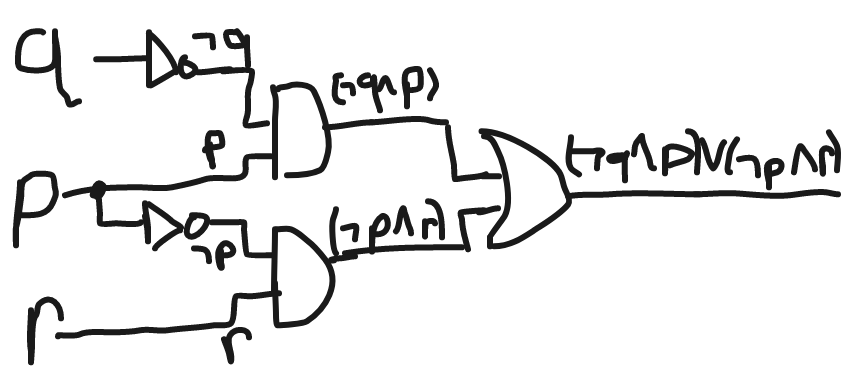
\includegraphics[scale=.545]{images/Prob6Solution.png}
\end{figure}
\section{Problem 7}
Are these system specification consistent?
Are these system specifications consistent? ``Whenever the system software is being upgraded, users cannot access the file system. If users can access the file system, then they can save new files. If users cannot save new files, then the system software is not being upgraded.''
\subsection{Solution}
System is \textbf{consistent}
\subsubsection{Explanation}
Let:\\
\indent u: \emph{``The system is being upgraded''}\\
\indent f: \emph{``Users can access the file system''}\\
\indent s: \emph{``Users are able to save new files''}\\
Rewrite the specifications as:
\begin{enumerate}[nosep, label=\arabic*)]
\item $u \rightarrow \neg f$
\item $f \rightarrow s$
\item $\neg s \rightarrow \neg u$
\end{enumerate}
Ley $u$ be true. This means that $\neg u$ is false. By the third statement, we know that $\neg s$ must be false in order to keep the statement true, meaning that $s$ must be true. By the first statement, we know that $\neg f$ must be true in order to keep the statement true, meaning that $f$ is false. Statement 2 is then $\textbf{F} \rightarrow \textbf{T} \equiv \textbf{T}$.\\
Since there exists a configuration of the system where each statement is true, the system must be consistent.
\section{Problem 8}
Write a negation for the statement:\\
There exists a real number $x$ such that $-2 \leq x < 4$.
\subsection{Solution}
For all real numbers $x$, $x < -2$ or $x \geq 4$.
\subsubsection{Explanation}
Note that we can rewrite the original statement symbolically as $(\exists x \in \mathbb{R})((-2 \leq x) \land (x < 4))$.\\
Using logical equivalences as shown below, we can rewrite the negation of the statement.\\
\begin{align*}
\neg (\exists x \in \mathbb{R})((-2 \leq x) \land (x < 4))
&\equiv (\forall x \in \mathbb{R})\neg((-2 \leq x) \land (x < 4)) && \text{(De Morgan's Law of Quantifiers)}\\
&\equiv (\forall x \in \mathbb{R})(\neg(-2 \leq x) \lor \neg(x < 4)) && \text{(De Morgan's Law of Propositional Logic)}\\
&\equiv (\forall x \in \mathbb{R})((x < -2) \lor (x \geq 4)) && \text{(Definition of Inequalities)}\\
\end{align*}
Note here that the definition of inequalities was used to reason about the idea that if $x$ is not greater than or equal to $-2$, then it must be less than $-2$ and that if $x$ is not less than $4$, then it must be greater than or equal to $4$.\\
Rewriting it in words, the negation of the initial statment is: ``For all real numbers $x$, $x < -2$ or $x \geq 4$.''
\section{Problem 9}
A sequence $a_n$ of real numbers converges if and only if\\
$\exists a \in \mathbb{R}, \forall \varepsilon > 0, \exists N \in \mathbb{Z},$ such that if $n \geq N,$ then $|a_n - a| < \varepsilon$.\\
Write the negation for this statement. That is, write what it means for the sequence $a_n$ to not converge.
\subsection{Solution}
A sequence $a_n$ of real numbers does not converge if and only if\\
$\forall a \in \mathbb{R}, \exists \varepsilon > 0$, such that $\forall N \in \mathbb{Z}, \exists n \in \mathbb{Z}$, such that $n \geq N$ and $|a_n - a| \geq \varepsilon$.
\subsubsection{Explanation}
Note that the second part of the original statement can be fully symbolically as\\
$\exists a \in \mathbb{R}, \forall \varepsilon > 0, \exists N \in Z, \forall n \in Z, (n \geq N) \rightarrow (|a_n-a| < \varepsilon)$.\\
Additionally, note that the implicit quantifier $\forall n \in Z$ was added to the definition in order to properly negate the statement.\\
Using logical equivalences as shown below, we can rewrite the negation of the statement. Note that ``DMQ'' denotes De Morgan's Law of Quantifiers.
\small
\begin{align*}
\neg \exists a \in \mathbb{R}, \forall \varepsilon > 0, \exists N \in Z, \forall n \in Z, (n \geq N) \rightarrow (|a_n-a| < \varepsilon)
&\equiv \forall a \in \mathbb{R}, \neg \forall \varepsilon > 0, \exists N \in Z, \forall n \in Z,\\&(n \geq N) \rightarrow (|a_n-a| < \varepsilon) && \text{(DMQ)}\\
&\equiv \forall a \in \mathbb{R}, \exists \varepsilon > 0, \neg \exists N \in Z, \forall n \in Z,\\&(n \geq N) \rightarrow (|a_n-a| < \varepsilon) && \text{(DMQ)}\\
&\equiv \forall a \in \mathbb{R}, \exists \varepsilon > 0, \forall N \in Z, \neg \forall n \in Z,\\&(n \geq N) \rightarrow (|a_n-a| < \varepsilon) && \text{(DMQ)}\\
&\equiv \forall a \in \mathbb{R}, \exists \varepsilon > 0, \forall N \in Z, \exists n \in Z,\\&\neg((n \geq N) \rightarrow (|a_n-a| < \varepsilon)) && \text{(DMQ)}\\
&\equiv \forall a \in \mathbb{R}, \exists \varepsilon > 0, \forall N \in Z, \exists n \in Z,\\&(n \geq N) \land \neg(|a_n-a| < \varepsilon) && \text{($\neg (p \rightarrow q) \equiv p \land \neg q)$)}\\
&\equiv \forall a \in \mathbb{R}, \exists \varepsilon > 0, \forall N \in Z, \exists n \in Z,\\&(n \geq N) \land (|a_n-a| \geq \varepsilon) && \text{(Definition of Inequality)}\\
\end{align*}
\normalsize
Note that the definition of inequality was used to reason that if $|a_n-a|$ is not less than $\varepsilon$, then it must be greater than or equal to $\varepsilon$.\\
Rewritten to match the style of the original statement, the negation of the second part of the original statement is: $\forall a \in \mathbb{R}, \exists \varepsilon > 0$, such that $\forall N \in \mathbb{Z}, \exists n \in \mathbb{Z}$, such that $n \geq N$ and $|a_n - a| \geq \varepsilon$.
\section{Problem 10}
Use symbols to write the logical form of the argument, and then use a truth table to test the argument for validity. State whether the argument is valid or invalid. Justify your conclusion in a sentence.
Oleg is a math major or Oleg is an economics major.\\
If Oleg is a math major, then Oleg is required to take Math 73.\\
$\therefore$Oleg is an economics major or Oleg is required to take Math 73.
\subsection{Solution}
Let $p$ be the statement Oleg is a math major.\\
Let $q$ be the statement Oleg is an economics major.\\
Let $r$ be the statement Oleg is required to take Math 73.\\
The premises can then be written as $p \lor q$ and $p \rightarrow r$. The conclusion can be written as $q \lor r$
\begin{displaymath}
\begin{array}{|c c c|c|c|c|}
p & q & r & p \lor q & p \rightarrow r & q \lor r\\
\hline
T & T & T & T & T & T\\
T & T & F & T & F & T\\
T & F & T & T & T & T\\
T & F & F & T & F & F\\
F & T & T & T & T & T\\
F & T & F & T & T & T\\
F & F & T & F & T & T\\
F & F & F & F & T & F\\
\end{array}
\end{displaymath}
Since every row that has both premises true has the conclusion true, the argument is valid.
\section{Problem 11}
Use the rules of inference to deduce the conclusion from the premises, giving a reason for each step.
\begin{gather*}
r \lor s\\
s \rightarrow p\\
r \land q \rightarrow t\\
\neg p\\
\neg s \rightarrow u \land q\\
\therefore t
\end{gather*}
Note that by operator precedence, one should rewrite the premises as the below to remove any confusion.
\begin{gather*}
r \lor s\\
s \rightarrow p\\
(r \land q) \rightarrow t\\
\neg p\\
\neg s \rightarrow (u \land q)\\
\therefore t
\end{gather*}
\subsection{Solution}
\begin{logicproof}{2}
r \lor s & Premise\\
s \rightarrow p & Premise\\
(r \land q) \rightarrow t & Premise\\
\neg p & Premise\\
\neg s \rightarrow (u \land q) & Premise\\
\neg s & Modus Tollens using (2), (4)\\
u \land q & Modus Ponens using (5), (6)\\
q & Simplifcation using (7)\\
r & Disjunctive Syllogism using (1), (6)\\
r \land q & Conjunction using (8), (9)\\
t & Modus Ponens using (3), (10)
\end{logicproof}
\section{Problem 12}
Are the following arguments valid or invalid? If the argument is valid, state whether Universal Modus Ponens, Universal Modus Tollens, or Universal Transitivity applies. More than one may apply. If the argument is invalid, state whether the converse or the inverse error
is made.
\begin{enumerate}[nosep, label=\alph*)]
\item All students can attend the dance.\\Sandra will attend the dance.\\Therefore, Sandra is student.
\item All students can attend the dance.\\Leo will not attend the dance.\\Therefore, Leo is not a student.
\item All students can attend the dance.\\Ms. Pumpernickel is not a student.\\Therefore, Ms. Pumpernickel cannot attend the dance.
\item All people are mice.\\All mice are mortal.\\Therefore, all people are mortal.
\item All discrete structures students can tell a valid argument from an invalid one.\\All thoughtful people can tell a valid argument from an invalid one.\\Therefore, all discrete mathematics students are thoughtful.
\end{enumerate}
\subsection{Solution}
\begin{enumerate}[nosep, label=\alph*)]
\item Invalid by converse error.
\item Valid by Universal Modus Tollens.
\item Invalid by inverse error.
\item Valid by Universal Transitivity.
\item Invalid by converse error (where the incorrect use of converse is that all thoughtful people can tell a valid argument from an invalid one is equivalent to all people able to tell valid arguments are thoughtful, which leads to an incorrect use of Universal Transitivity that states that all discrete structures people are thoughtful).
\end{enumerate}
\end{document}